% Submersión Espectral de Lenguajes Perdidos — versión consolidada a dos columnas
% Compilar: pdflatex (x2)
\documentclass[10pt,twocolumn]{article}

\usepackage[utf8]{inputenc}
\usepackage[T1]{fontenc}
\usepackage[spanish,es-nodecimaldot]{babel}
\usepackage{lmodern}
\usepackage{microtype}
\usepackage[a4paper,margin=1.9cm,columnsep=0.75cm]{geometry}
\usepackage{amsmath,amssymb,amsfonts,amsthm,mathtools}
\usepackage{bm}
\usepackage{booktabs}
\usepackage{graphicx}
\usepackage{float}
\usepackage{xcolor}
\usepackage{enumitem}
\usepackage{verse}
\usepackage[colorlinks=true,linkcolor=blue!50!black,citecolor=blue!50!black,urlcolor=blue!50!black]{hyperref}
\usepackage{caption}
\captionsetup{font=small,labelfont=bf}

\definecolor{madera}{HTML}{6B5A3E}

\newtheorem{theorem}{Teorema}[section]
\newtheorem{proposition}[theorem]{Proposición}
\newtheorem{definition}[theorem]{Definición}
\newtheorem{remark}[theorem]{Observación}

\setlength{\parskip}{2pt}

\title{\bfseries Submersión Espectral de Lenguajes Perdidos:\\
un marco auditable de generación de hipótesis\\
y un traductor simbólico hacia Rongorongo\\[4pt]
\large Versión consolidada v2}

\author{David Astudillo (SatisfyMath)\\
\small \texttt{satisfimath@gmail.com} \quad · \quad
\small repositorio: \texttt{github.com/satisfymath/spectral-submersion}}

\date{Agosto 2026}

\begin{document}

\twocolumn[{
\maketitle
\begin{center}
\begin{minipage}{0.86\textwidth}
\small
\textbf{Resumen.}
El desciframiento de sistemas de escritura no descifrados es un problema
inverso mal puesto en el sentido de Hadamard: sin anclajes externos, toda
estadística interna es invariante bajo permutaciones de los nombres de los
signos, y ningún algoritmo puede identificar una traducción absoluta desde
estructura pura. Este trabajo consolida un marco matemático
—co-ocurrencias, PMI/PPMI, descomposición espectral (SVD), alineamiento
Procrustes, transporte óptimo y submersiones entre variedades semánticas—
cuyo producto válido no es una traducción única sino una \emph{familia
auditada de hipótesis} con controles negativos, cotas de identificabilidad
parcial y análisis de estabilidad. Validamos el pipeline en benchmarks
sintéticos con gramática conocida (recuperación de anclajes con
Acc@1 $=68.9\%$ usando solo $20\%$ de pares), en el corpus real del valle
del Indo (sesgo posicional estructural: signos con $78\%$ de aparición
inicial frente a $\le 21\%$ en controles) y, como novedad de esta versión,
en el \textbf{corpus Rongorongo real} (tablillas A--F, 5\,460 glifos, 941
tipos en codificación Barthel). Sobre este corpus construimos un traductor
secuencia-a-secuencia (Transformer, 5.8M parámetros) desde glosas
rapanui hacia códigos Barthel auténticos, decodificado mediante beam
search con fusión superficial de un modelo de lenguaje trigrama entrenado
en las tablillas reales. La versión v6 alcanza $100\%$ de vocabulario
atestiguado, $71.5\%$ de bigramas atestiguados y 7.3 bits/glifo bajo el LM
real (cota held-out real: 8.26), eliminando la degeneración repetitiva de
versiones anteriores. Cerramos con una aplicación demostrativa
extremo-a-extremo: la inscripción de un poema dedicatorio en una tablilla
sintética con glifos Barthel reales. Todos los resultados distinguen
explícitamente entre \emph{señal estructural} (defendible) e
\emph{hipótesis semántica} (no verificable), y el código, los datos y los
manifiestos de reproducibilidad son públicos.\\[2pt]
\textbf{Palabras clave:} Rongorongo · desciframiento computacional ·
problemas inversos · SVD · transporte óptimo · Transformer · escritura del
Indo.
\end{minipage}
\end{center}
\vspace{14pt}
}]

\section{Introducción}

Los sistemas de escritura no descifrados —Rongorongo de Rapa Nui, la
escritura del valle del Indo, el Lineal A— comparten una condición
epistémica: existe abundante estructura estadística interna y ningún
puente verificado hacia una lengua conocida. La tentación histórica ha
sido saltar directamente de la estructura a la semántica; la posición de
este trabajo es que ese salto debe ser reemplazado por un \emph{marco de
generación de hipótesis auditable}, en el que cada afirmación lleva
adjunto su nivel de evidencia, sus controles negativos y sus límites de
identificabilidad.

Este documento consolida el trabajo acumulado del proyecto
\emph{Spectral Submersion}: (i) el marco matemático formal
(Sec.~\ref{sec:marco}); (ii) el programa experimental con benchmarks
sintéticos controlados y el corpus real del Indo
(Sec.~\ref{sec:experimentos}); (iii) la incorporación del corpus
Rongorongo real y el traductor simbólico v6
(Secs.~\ref{sec:corpus-real}--\ref{sec:v6}); y (iv) el protocolo de
niveles de afirmación (Sec.~\ref{sec:claims}). La
Sec.~\ref{sec:aplicacion} presenta la aplicación demostrativa final.

\section{Marco matemático}
\label{sec:marco}

\subsection{El desciframiento como problema inverso mal puesto}

Sea $X$ un corpus finito de signos no descifrados con vocabulario
$\mathcal{V}_X$, y sea $\mathcal{Y}$ una familia de corpus candidatos.
Definimos un operador de observación $\mathcal{O}:\Theta\to\mathcal{D}_X$
que envía cada hipótesis de correspondencia $\theta$ al conjunto de
estadísticas observables (frecuencias, co-ocurrencias, espectros). El
desciframiento exige invertir $\mathcal{O}$.

\begin{proposition}[Mal planteamiento]
\label{prop:hadamard}
El problema inverso del desciframiento no anclado viola las tres
condiciones de Hadamard: la existencia de una correspondencia léxica
simple no está garantizada; la unicidad falla por invariancia bajo el
grupo de permutaciones $S_{|\mathcal{V}_X|}$ actuando sobre los nombres de
los signos; y la estabilidad falla porque variaciones paleográficas
pequeñas alteran bigramas, grafos y embeddings.
\end{proposition}

\begin{theorem}[No-desciframiento gratuito]
\label{thm:nofree}
Sea $\sigma\in S_{|\mathcal{V}_X|}$ una permutación de etiquetas de
signos. Toda estadística interna invariante bajo re-etiquetado satisface
$\mathcal{O}(\theta)=\mathcal{O}(\sigma\circ\theta)$. En consecuencia,
ningún algoritmo que consuma únicamente estadísticas internas de $X$
puede distinguir $\theta$ de $\sigma\circ\theta$: la identificabilidad
absoluta requiere anclajes externos $K$.
\end{theorem}

La versión completa de las demostraciones se encuentra en el manuscrito
extendido del proyecto \cite{astudillo2026}. El corolario operativo es la
reformulación del objetivo científico como distribución posterior
\begin{equation}
p\!\left(x_{1:T}\mid y_{1:M},K\right),
\label{eq:posterior}
\end{equation}
donde $y_{1:M}$ es una entrada rapanui/polinesia, $x_{1:T}$ una secuencia
glífica candidata y $K$ el conocimiento externo documentado (paleografía,
orientación, calendario, tradición oral, iconografía).

\subsection{Pipeline espectral}

Del corpus se construye la matriz de co-ocurrencia ventanal $C$ (con
respeto de fronteras de línea), la matriz PPMI
$M_{ij}=\max\{0,\log\frac{p_{ij}}{p_i p_j}\}$ y su SVD truncada
$M\approx U_k\Sigma_k V_k^{\top}$, que define embeddings
$E=U_k\Sigma_k^{\alpha}$. Tres resultados clásicos sostienen el pipeline:
la optimalidad de rango bajo de Eckart--Young--Mirsky, la solución
cerrada del alineamiento ortogonal de Procrustes
$\Omega^{*}=UV^{\top}$ con $U\Sigma V^{\top}=\mathrm{svd}(A^{\top}B)$, y
la contracción espectral de la regularización de Tikhonov
$\sigma\mapsto\sigma/(\sigma^2+\lambda)$, que acota la amplificación de
ruido en la pseudoinversa. Para comparar espacios de distinto tamaño se
emplea transporte óptimo entrópico (Sinkhorn) y distorsión relacional
tipo Gromov--Wasserstein.

\begin{definition}[Rango efectivo]
Para valores singulares $\sigma_1\ge\dots\ge\sigma_k$, con
$p_i=\sigma_i/\sum_j\sigma_j$, el rango efectivo es
$r_{\mathrm{eff}}=\exp\!\big(-\sum_i p_i\log p_i\big)$.
\end{definition}

El rango efectivo funciona como detector de estructura: corpus con
gramática subyacente comprimen ($r_{\mathrm{eff}}$ bajo) mientras que sus
controles aleatorizados no.

\section{Programa experimental}
\label{sec:experimentos}

\subsection{Controles negativos en benchmark sintético}

Sobre un corpus PCFG de 112 tipos y $\sim$24k tokens con gramática
conocida, el corpus real comprime a $r_{\mathrm{eff}}=11.18$ frente a
$13.9$--$14.2$ de los tres controles (permutado, aleatorio con mismas
frecuencias, uniforme; Tabla~\ref{tab:controles}). El bootstrap (50
remuestreos) da un coeficiente de variación del rango efectivo de
$0.65\%$ y similitud coseno media entre embeddings de $0.77$: la
geometría es estable, no un artefacto de muestreo.

\begin{table}[t]
\centering
\small
\caption{Controles negativos, corpus sintético rico (112 tipos).}
\label{tab:controles}
\begin{tabular}{lccc}
\toprule
Variante & $r_{\mathrm{eff}}$ & $\sigma_1$ & $\sum\sigma$\\
\midrule
real & \textbf{11.18} & 31.79 & 139.98\\
permutado & 14.18 & 16.34 & 78.59\\
aleatorio (mismas frec.) & 14.15 & 16.99 & 80.88\\
aleatorio uniforme & 13.91 & 13.72 & 61.61\\
\bottomrule
\end{tabular}
\end{table}

\subsection{Recuperación de anclajes bajo isometría}

Cuando las premisas de identificabilidad parcial se satisfacen
(permutación exacta conocida sobre 112 pares, $20\%$ de anclajes de
entrenamiento), Procrustes recupera la correspondencia de test con
Acc@1 $=0.689$, Acc@5 $=0.833$, MRR $=0.760$ y rango mediano 1. Esto
valida el algoritmo \emph{condicionado a sus premisas}; no implica
rendimiento equivalente en datos arqueológicos donde estas no se cumplen.

\subsection{Sesgo posicional en el corpus Indo real}

En el corpus real del Indo (179 inscripciones, 182 signos), los signos
P324 y P217 aparecen en posición inicial el $78\%$ de las veces y P385 en
posición final el $83\%$, frente a $\le 21\%$ en los tres controles
negativos (Fig.~\ref{fig:posicional}); la detección de comunidades
(Louvain sobre red PPMI) agrupa los signos iniciales en una misma
comunidad. Un benchmark sintético con sesgo posicional diseñado (TITLE
$80\%$ inicial, NUMERAL $80\%$ final) confirma que la métrica detecta las
clases correctas sin falsos positivos. Estos hallazgos replican de forma
independiente la literatura epigráfica del Indo y constituyen
\emph{señal estructural} en el sentido de la Sec.~\ref{sec:claims}.

\begin{figure}[t]
\centering
\includegraphics[width=\linewidth]{reports/figures/paper_fig1_positional_bias.pdf}
\caption{Sesgo posicional en el corpus Indo real frente a controles
negativos. Las diferencias real--control superan $+0.6$ en ratio de
posición.}
\label{fig:posicional}
\end{figure}

\begin{figure}[t]
\centering
\includegraphics[width=\linewidth]{reports/figures/paper_fig2_entropy_curves.pdf}
\caption{Curvas de entropía condicional por tamaño de contexto (estilo
Rao et al.), comparando corpus reales, sintéticos y controles.}
\label{fig:entropia}
\end{figure}

\subsection{Honestidad del pipeline: sanity checks fallidos}

Documentamos también los negativos: en corpus de vocabulario grande y
secuencias cortas (Indo real; sintéticos tipo Rongorongo), el chequeo
espectral $r_{\mathrm{eff}}^{\mathrm{real}}<r_{\mathrm{eff}}^{\mathrm{unif}}$
falla incluso con hiperparámetros calibrados por búsqueda en malla (96
configuraciones). La co-ocurrencia ventanal es insuficiente allí donde la
estructura es principalmente posicional; el análisis posicional es el
instrumento correcto. Reportar estos fallos es parte del diseño del
marco.

\section{El corpus Rongorongo real}
\label{sec:corpus-real}

Versiones anteriores del proyecto documentaron la ausencia de
transcripciones normalizadas públicas de Rongorongo. Esta versión
incorpora el corpus RR (transcripción phspaelti) para las tablillas
A--F, convertido a formato tabular normalizado:
6 tablillas, 107 líneas, \textbf{5\,460 glifos}, \textbf{941 tipos} en
codificación numérica de Barthel (razón tipo/token $0.172$), con
marcadores de ligadura y variante preservados como parte del token. La
distribución de frecuencias es fuertemente zipfiana: los códigos
geométricos simples (001, 002, 004, 006) dominan, seguidos por las
series antropomorfa (200--399), aviforme (600--699, encabezada por la
fragata 600) e ictiomorfa (700--799).

Sobre este corpus entrenamos un modelo de lenguaje trigrama con
interpolación y suavizado aditivo
($\lambda_3{=}0.5,\lambda_2{=}0.3,\lambda_1{=}0.2$, $k{=}0.1$), que
constituye tanto el instrumento de evaluación como el componente de
fusión del decodificador (Sec.~\ref{sec:v6}). La entropía cruzada de
líneas reales held-out (tablillas D y F bajo un LM entrenado en A, B, C y
E) es de \textbf{8.26 bits/glifo}, y define la cota de referencia de
realismo secuencial.

\section{Traductor simbólico v6}
\label{sec:v6}

\subsection{Corpus paralelo anclado en glifos reales}

No existe corpus paralelo rapanui--Rongorongo verificado; por el
Teorema~\ref{thm:nofree} ninguna construcción interna puede producirlo.
Construimos en su lugar un corpus paralelo \emph{sintético anclado}:
60\,000 pares glosa-rapanui $\to$ secuencia Barthel, donde la selección
de glifos está (i) restringida por una correspondencia
categoría$\to$rango de Barthel declarada explícitamente como
\emph{hipótesis de trabajo} (determinantes/partículas $\to$ 001--099;
nombres y sustantivos de persona $\to$ 200--399; verbos $\to$ 400--599;
dominio aviar $\to$ 600--699; dominio marino $\to$ 700--799), (ii)
ponderada por la frecuencia unigrama real dentro de cada clase y (iii)
suavizada por transiciones bigrama reales (con probabilidad 0.45 el
glifo se remuestrea de $P(g\mid g_{\mathrm{prev}})$ restringido a la
clase). El proceso de reduplicación observado en las tablillas se modela
explícitamente ($12\%$ duplicación, $3\%$ triplicación). El corpus
resultante cubre 939 de los 941 tipos reales.

\subsection{Arquitectura y decodificación}

El traductor es un Transformer encoder-decoder (4+4 capas,
$d_{\mathrm{model}}{=}256$, 8 cabezas, FFN 512; 5.8M parámetros)
entrenado 15 épocas con AdamW, recocido coseno y aumento de datos por
enmascaramiento ($\mathrm{PPL}_{\mathrm{val}}$: $51.9\to10.74$). La
decodificación es beam search ($B{=}5$) con \emph{fusión superficial}
del LM real:
\begin{equation}
s(y)=(1-\lambda)\log p_{\mathrm{model}}(y\mid x)+\lambda\log
p_{\mathrm{LM}}(y),
\end{equation}
con $\lambda=0.35$, normalización por longitud y penalización de la
tercera repetición inmediata (la duplicación es rasgo real; las rachas
largas son degeneración).

\subsection{Evaluación}

La Tabla~\ref{tab:eval} y la Fig.~\ref{fig:eval} comparan v5 (códigos
sintéticos, decodificación voraz) con v6 en sus dos modos, sobre 20
oraciones de test. El modo beam+fusión domina en todos los ejes
relevantes: vocabulario $100\%$ atestiguado, $71.5\%$ de bigramas
atestiguados en las tablillas, divergencia JS unigrama mínima frente al
corpus real, diversidad distinct-2 de $0.72$ y racha máxima de
repetición 2 —exactamente el patrón de reduplicación real—, frente a
rachas degeneradas de 48--50 en los modos voraces. Su entropía cruzada
bajo el LM real (7.31 bits/glifo) queda por debajo de la cota held-out
real (8.26), como corresponde a un generador más predecible que el
texto genuino.

\begin{table}[t]
\centering
\small
\caption{Evaluación frente a estadísticas del corpus real (20 oraciones
de test). VR: vocabulario real; BA: bigramas atestiguados; JS:
divergencia Jensen--Shannon unigrama; D2: distinct-2; RM: racha máxima
de repetición; b/g: bits/glifo bajo el LM real.}
\label{tab:eval}
\begin{tabular}{lcccccc}
\toprule
Sistema & VR & BA & JS & D2 & RM & b/g\\
\midrule
v5 voraz & 0\% & 0\% & 1.00 & 0.44 & 48 & ---\\
v6 voraz & 100\% & \textbf{86.6\%} & 0.54 & 0.19 & 50 & \textbf{7.21}\\
v6 beam+fusión & 100\% & 71.5\% & \textbf{0.52} & \textbf{0.72} & \textbf{2} & 7.31\\
\midrule
real held-out & --- & --- & --- & --- & --- & 8.26\\
\bottomrule
\end{tabular}
\end{table}

\begin{figure*}[t]
\centering
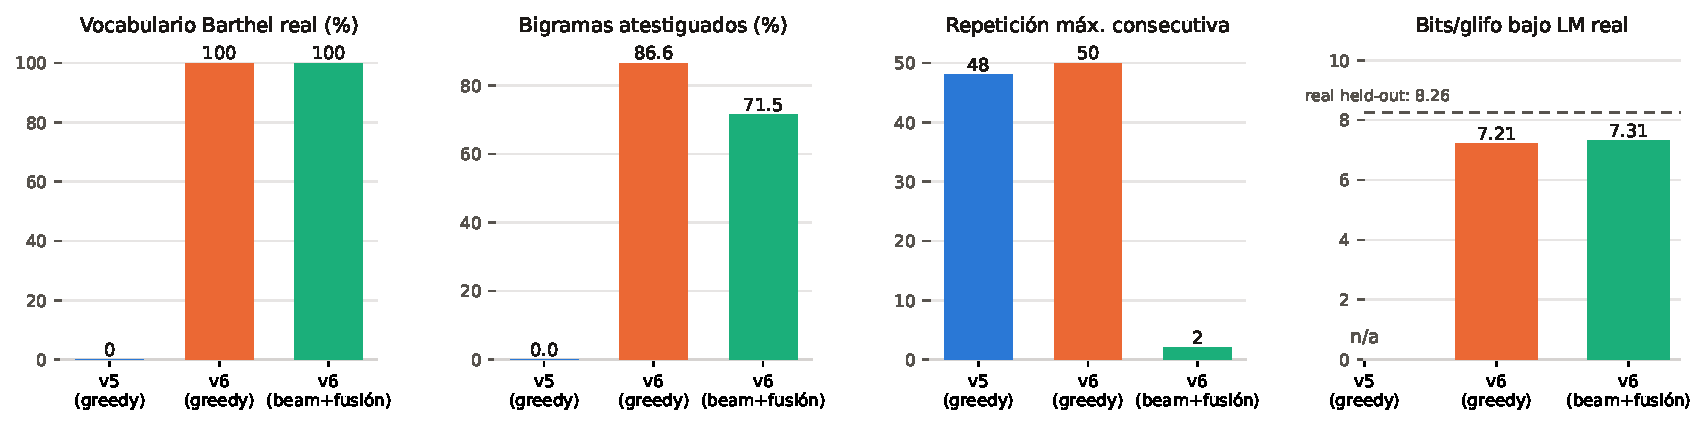
\includegraphics[width=\textwidth]{reports/figures/paper_fig5_v6_eval.pdf}
\caption{Evaluación de los tres sistemas frente al corpus Rongorongo
real. De izquierda a derecha: fracción de vocabulario Barthel
atestiguado; fracción de bigramas atestiguados; racha máxima de
repetición inmediata (la duplicación es rasgo real, las rachas largas
son degeneración); entropía cruzada bajo el LM trigrama real, con la
cota held-out real como referencia.}
\label{fig:eval}
\end{figure*}

\section{Niveles de afirmación y limitaciones}
\label{sec:claims}

El marco distingue tres niveles: \textbf{C1, señal estructural}
(defendible con controles negativos: compresión espectral, sesgo
posicional, comunidades); \textbf{C2, hipótesis de correspondencia}
(rankeable, no verificable: la asignación categoría$\to$rango Barthel, los
candidatos icónicos); \textbf{C3, traducción semántica} (no admisible con
la evidencia actual). El traductor v6 opera íntegramente en C2: sus
salidas son \emph{plausibles bajo las estadísticas reales}, no
\emph{correctas}. El benchmark icónico cross-script del proyecto
(jeroglíficos egipcios y signos chinos con referente conocido) no superó
el umbral C2.5, lo que refuerza mantener los anclajes icónicos en nivel
de hipótesis. Limitaciones adicionales: el corpus paralelo es sintético
por necesidad lógica; la glosa rapanui usa un léxico restringido de 232
tipos; y la transcripción Barthel hereda las decisiones paleográficas de
su fuente.

\section{Aplicación demostrativa y dedicatoria}
\label{sec:aplicacion}

Como demostración extremo-a-extremo del sistema completo —glosa,
traducción v6 beam+fusión, y renderizado con los trazados vectoriales de
glifos reales del corpus RR en bustrofedón inverso— inscribimos un poema.
Las diez líneas núcleo, su glosa rapanui y su secuencia Barthel se listan
en la Tabla~\ref{tab:poema}; la tablilla resultante es la
Fig.~\ref{fig:tablilla}. Cada línea obtiene entre 6.1 y 7.2 bits/glifo
bajo el LM real, dentro de la cota de realismo. Obsérvese la
estructura espejo de L5 (\emph{eres calma y también incendio}:
$002\,002\cdots700\,700\cdots001\,001$) y la fórmula recurrente
$041h\,670\,580$ que el modelo asocia al verbo \emph{makemake}
(desear/elegir) —que es, además, el nombre del dios creador rapanui.

\begin{table*}[t]
\centering
\small
\caption{«La mejor posibilidad» destilada: verso, glosa rapanui y
secuencia Barthel (v6 beam+fusión). b/g: bits/glifo bajo el LM real.}
\label{tab:poema}
\scriptsize
\begin{tabular}{cp{4.1cm}p{4.6cm}p{5.6cm}c}
\toprule
L & Verso & Glosa rapanui & Secuencia Barthel & b/g\\
\midrule
1 & nos enamoramos antes de saber & \emph{e aroha taua i mua o te kite} & 002 002 700 408 002 002 700 001 001 006 430 & 6.41\\
2 & lo mejor que me ha pasado & \emph{ko kou te hua reka o taku ora} & 002 002 010 700 700 004 004 002 595 & 6.22\\
3 & llegaste a acompañarme & \emph{e haere kou ma au, e haere taua tahi} & 002 002 700 700 408 092 001 001 006 400 004 004 002 002 & 6.33\\
4 & un hogar es una persona & \emph{taku hare ko kou} & 004a 064a 001 001 & 7.18\\
5 & eres calma y también incendio & \emph{ko kou te hau, ko kou te hana} & 002 002 010 010 700 700 001 001 006 430 & 6.27\\
6 & las ganas de elegirte & \emph{makemake au ki a kou i te rau raa} & 041h 670 580 001 006 006 074f 011 741 & 7.24\\
7 & puedes volar y aun así regresas & \emph{e rere kou, e hoki mai kou} & 002 002 123 430 022 002 002 & 6.17\\
8 & materia del universo que se encontró & \emph{te take o taua no te rangi} & 005 065 065 003 002 002 010 205 & 6.37\\
9 & quiero conocerte toda la vida & \emph{makemake au kite ki a kou i te ora tonu} & 041h 670 580 001 004 004 002 002 004 004 430 022 & 6.30\\
10 & la vida que siga construyendo contigo & \emph{te ora e haere ki mua ma kou} & 005 670 580 004 004 760 004 002 002 & 6.44\\
\bottomrule
\end{tabular}
\end{table*}

\begin{figure*}[t]
\centering
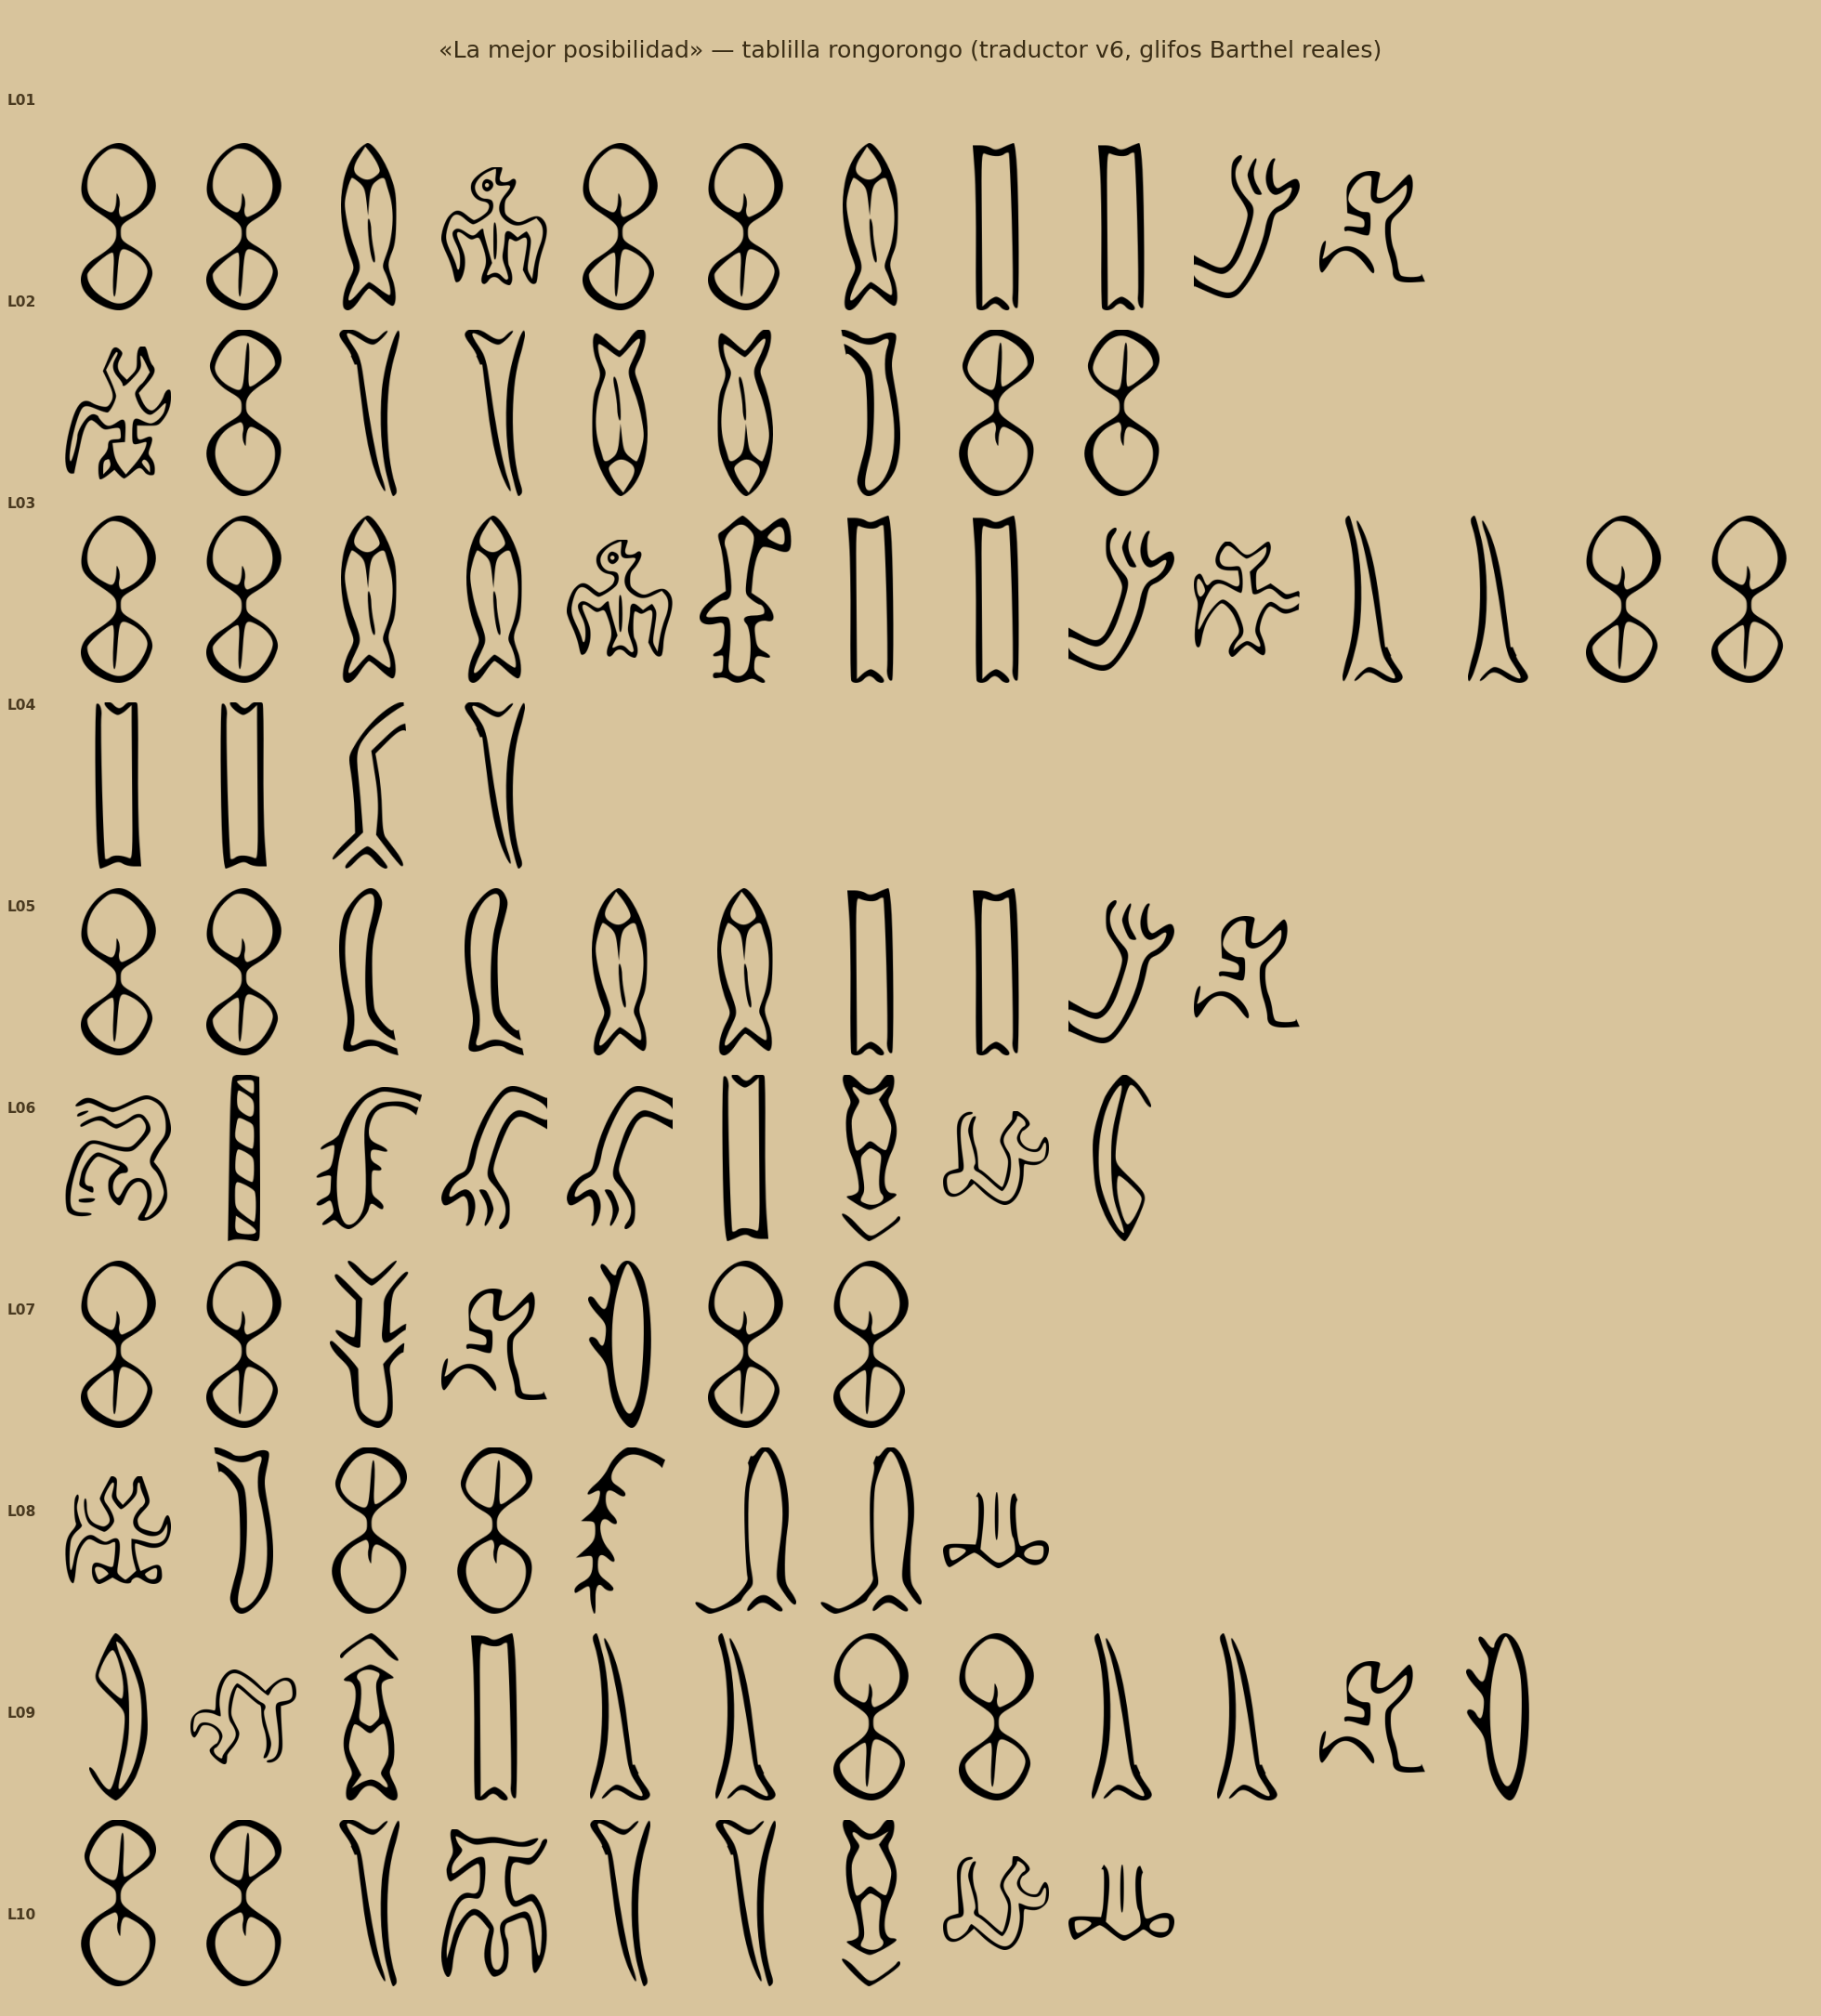
\includegraphics[width=0.92\textwidth]{reports/figures/tablilla_mejor_posibilidad.png}
\caption{Tablilla sintética de «La mejor posibilidad»: diez líneas en
bustrofedón inverso (líneas pares rotadas $180^{\circ}$), compuestas con
los trazados vectoriales de glifos reales del corpus RR. Salida del
traductor v6 con beam search y fusión del LM real.}
\label{fig:tablilla}
\end{figure*}

\subsection*{Dedicatoria}

\begin{center}
\itshape
Para María Ignacia Xerra,\\
mi futura esposa.\\[6pt]
\normalfont\small
Entre todas las combinaciones posibles de esta absurda realidad,\\
el caos terminó formando tus ojos,\\
y entre millones de secuencias glíficas posibles,\\
todas las de esta tablilla dicen lo mismo:\\[4pt]
\itshape te ora e haere ki mua ma kou —\\
la vida que siga construyendo contigo.
\end{center}

\section*{Reproducibilidad}

Código, configuraciones, manifiestos con sumas SHA-256 y datos públicos
en \url{https://github.com/satisfymath/spectral-submersion}. Los scripts
relevantes de esta versión: \texttt{generate\_massive\_parallel\_v4.py}
(corpus paralelo anclado), \texttt{translate\_to\_rongorongo\_v6.py}
(beam + fusión LM), \texttt{evaluate\_rongorongo\_v6.py} (evaluación
contra el corpus real).

\begin{thebibliography}{9}\small

\bibitem{astudillo2026} D. Astudillo.
\emph{Submersión espectral de lenguajes perdidos} (manuscrito extendido
del proyecto), 2026.

\bibitem{barthel} T. Barthel.
\emph{Grundlagen zur Entzifferung der Osterinselschrift}. Cram, de
Gruyter \& Co., 1958.

\bibitem{rao} R. Rao, N. Yadav, M. Vahia, H. Joglekar, R. Adhikari,
I. Mahadevan. Entropic evidence for linguistic structure in the Indus
script. \emph{Science} 324(5931), 2009.

\bibitem{pozdniakov} K. Pozdniakov, I. Pozdniakov. Rapanui writing and
the Rapanui language: preliminary results of a statistical analysis.
\emph{Forum for Anthropology and Culture} 3, 2007.

\bibitem{horley} P. Horley. Allographic variation and statistical
analysis of the Rongorongo script. \emph{Rapa Nui Journal} 19(2), 2005.

\bibitem{eckart} C. Eckart, G. Young. The approximation of one matrix by
another of lower rank. \emph{Psychometrika} 1, 1936.

\bibitem{cuturi} M. Cuturi. Sinkhorn distances: lightspeed computation
of optimal transport. \emph{NeurIPS}, 2013.

\bibitem{gulcehre} C. Gulcehre et al. On using monolingual corpora in
neural machine translation. \emph{arXiv:1503.03535}, 2015.

\bibitem{parpola} A. Parpola. \emph{Deciphering the Indus Script}.
Cambridge University Press, 1994.

\end{thebibliography}

\onecolumn
\appendix
\section{El poema completo}
\label{app:poema}

{\small\itshape
\setlength{\parskip}{3pt}
\noindent\textbf{\upshape LA MEJOR POSIBILIDAD}\\[6pt]
Éramos jóvenes, / y quizás por eso no entendíamos / la magnitud de lo que
nos estaba pasando. // Nos enamoramos antes de saber / que estábamos
enamorados. // Como dos cuerpos que descubren la gravedad / mucho antes
de conocer su nombre. // Y ahora pienso / en todas las pequeñas
decisiones, / en todos los accidentes, / en todas las coincidencias
improbables / que tuvieron que ocurrir / para que tú y yo / termináramos
aquí. // Y me parece una locura. / Una hermosa locura. // Porque entre
millones de personas, / entre todas las vidas que pude haber vivido, /
todos los lugares donde pude haber estado / y todas las personas que pude
haber conocido, / \textbf{me pasó la vida contigo.} // Y eso es, sin
exagerar, / lo mejor que me ha pasado.

\noindent No llegaste a salvarme. / Llegaste a algo mucho más hermoso: /
\textbf{a acompañarme.} / A caminar conmigo / sin pedirme que dejara de
ser quien soy. // A hacerme entender / que la estabilidad no tiene por
qué ser aburrida, / que también puede tener música, / deseo, / viajes
improvisados, / risas estúpidas a las tres de la mañana / y besos que
hacen perder completamente la razón. // Contigo descubrí / que tener un
hogar / no siempre significa tener cuatro paredes. // A veces un hogar /
es una persona. / Una voz. / Un abrazo. / Una forma particular / de decir
mi nombre. // A veces el hogar / es saber que el mundo puede estar
ardiendo afuera / y aun así sentir paz / porque estás acostada a mi lado.

\noindent\textbf{\upshape Coro.} Porque tú eres calma / y también eres
incendio. // Eres el lugar donde descanso / y las ganas que tengo de
salir corriendo / a conquistar el mundo. // Eres confort, / pero nunca
conformismo. / Eres estabilidad, / pero jamás monotonía. // Eres esa paz
extraña / que al mismo tiempo / me vuelve completamente loco. // Y yo
quiero vivirlo todo contigo. / Quiero los días grandes / y los días
insignificantes. / Las victorias, / los domingos, / los viajes, / las
noches largas, / los desayunos medio dormidos. // Quiero desearte cuando
tengamos veinte, / treinta, / cuarenta / y cuando nuestros cuerpos /
empiecen lentamente / a contar la historia de que vivimos. // Porque de
todo lo que puedo perder con el tiempo, / hay algo que quiero conservar
intacto: / \textbf{las ganas de elegirte.}

\noindent Tú me das ganas. / Y creo que eso / es una de las formas más
hermosas del amor. // Ganas de hacer cosas. / Ganas de levantarme. /
Ganas de construir. / Ganas de viajar. / Ganas de llegar más lejos. /
Ganas de volver a casa / para contarte lo que pasó. / Ganas de mostrarte
algo / cuando descubro algo nuevo. / Ganas de pensar en el futuro / sin
sentir que el futuro pesa. // Antes mis sueños eran míos. / Ahora hay
sueños / en los que apareces tú, / y extrañamente / no siento que haya
perdido libertad. / Siento que mi mundo se hizo más grande. // Porque
amar bien / no debería reducir nuestras posibilidades. / Debería
multiplicarlas. // Y tú hiciste eso conmigo. / No cerraste puertas. /
Abriste ventanas / que ni siquiera sabía que existían.

\noindent Hay algo profundamente hermoso / en saber que ninguno de los
dos / está obligado a estar aquí. // Somos libres. / Podríamos elegir
otros caminos. / Podríamos construir otras vidas. / Y sin embargo, /
entre toda esa inmensidad de posibilidades, / nos miramos / y seguimos
diciendo: / \textbf{tú.} // Eso para mí es amor. / No necesitar cadenas /
para permanecer juntos. / No necesitar promesas imposibles / para
confiar. / Saber que puedes volar / y aun así quieres regresar. / Saber
que yo también puedo hacerlo / y que mi lugar favorito / sigue siendo
contigo.

\noindent Te miro / y todavía existe deseo. / Ese deseo animal, /
absurdo, / eléctrico. / Las ganas de besarte / como si acabara de
conocerte. // Pero también existe algo / mucho más profundo: / después
del fuego, / quiero quedarme. / Quiero abrazarte. / Quiero dormir
contigo. / Quiero despertar / y encontrarte todavía ahí. // Y quizás esa
sea / mi definición favorita del amor: / \textbf{tener ganas de devorarte
/ y al mismo tiempo / querer cuidarte toda la vida.}

\noindent A veces pienso / que somos materia intentando comprenderse. /
Un montón de átomos / que durante miles de millones de años / viajaron
por el universo / para terminar formando nuestros cuerpos. // Y míranos
ahora. / Tus manos tocando las mías. / Tu cabeza sobre mi pecho. / Yo
riéndome contigo / por alguna estupidez. // Es ridículamente improbable.
/ Y justamente por eso / me parece extraordinario. // Quizás el universo
no tenga intención. / Quizás todo sea azar. / Pero si todo esto fue
simplemente azar, / entonces tuve / una suerte inconcebible. // Porque el
caos / terminó formando tus ojos. / El tiempo / terminó cruzando nuestras
historias. / Y entre todas las combinaciones posibles / de esta absurda
realidad, / yo terminé amándote a ti.

\noindent\textbf{\upshape Puente.} Y quiero empujarte siempre hacia
arriba. / Nunca delante de mí. / Nunca detrás. / A mi lado. // Quiero
celebrar tus victorias / como si fueran también un poco mías. / Quiero
verte convertirte / en todo lo que quieras ser. / Quiero recordarte quién
eres / cuando tengas días / en que tú misma lo olvides. // Quiero que
tengas sueños / que no me incluyan. / Quiero que tengas mundos propios. /
Ideas propias. / Locuras propias. / Y aun así quiero ser / la primera
persona / a la que quieras correr a contarle / cuando algo maravilloso
suceda. // Porque no quiero poseerte. / \textbf{Quiero conocerte durante
toda la vida.} / Quiero verte cambiar. / Quiero enamorarme / de todas las
mujeres / en las que te vas a convertir. / Y que tú conozcas también /
todas las versiones que todavía faltan de mí.

\noindent No sé exactamente / qué nos espera. / Nadie puede saberlo. / El
tiempo es inexorable. / Avanza. / Nos cambia. / Se lleva cosas. / Nos
entrega otras. // Y por mucho que nos creamos dioses / capaces de
controlar nuestra existencia, / hay cosas / que simplemente suceden. /
Como tú. / \textbf{Tú me sucediste.} / Sin estrategia. / Sin cálculo. /
Sin pedir permiso. / Y cambiaste completamente / la geometría de mi
vida. / De pronto había un nosotros. / Un punto de referencia. / Un lugar
al cual regresar.

\noindent Yo antes pensaba / que una vida extraordinaria / tenía que
estar llena / de acontecimientos extraordinarios. / Ahora no. / Ahora
pienso / que quizás una buena vida / se construye acumulando pequeñas
cosas: / tu risa desde otra pieza, / un beso antes de salir, / una
conversación que dura demasiado, / tu mano buscando la mía, / hacer
planes imposibles, / comprar algo juntos, / perdernos, / volver, /
reconciliarnos, / reírnos, / desearnos, / crecer. // Quizás la felicidad
/ no sea un momento gigantesco. / Quizás sea mirar hacia atrás algún día
/ y descubrir / que estuvimos construyéndola / sin darnos cuenta.

\noindent\textbf{\upshape Final.} Así que esta es mi promesa. / No voy a
prometerte perfección. / Prefiero prometerte verdad. // Prometo seguir
teniendo ganas. / Ganas de nosotros. / Ganas de sorprenderte. / Ganas de
cuidarte. / Ganas de hacerte reír. / Ganas de construir. / Ganas de
discutir ideas contigo / hasta que ninguno recuerde / cómo empezó la
conversación. / Ganas de viajar. / Ganas de volver. / Ganas de hacer
locuras. / Ganas de darte paz. / Ganas de verte crecer. / Ganas de crecer
contigo. // Y cuando la vida se vuelva difícil, / porque alguna vez lo
hará, / recordar que no solamente somos amor. / Somos equipo. / Somos
refugio. / Somos deseo. / Somos impulso. / Somos libertad. / Somos
estabilidad. // Somos dos personas / que tuvieron la increíble fortuna /
de encontrarse / y la inteligencia emocional / de decidir construirse. //
Y si algún día me preguntan / cuál fue la decisión más importante de mi
vida, / no voy a decir un trabajo, / un lugar, / un logro / ni alguna
cifra. / Voy a pensar en ti. // Porque después de todo lo vivido / hay
una certeza / que no necesito analizar: / \textbf{tú eres lo mejor que me
ha pasado en la vida.} // Mi paz / sin quitarme la locura. / Mi
estabilidad / sin quitarme las ganas de volar. / Mi deseo. / Mi
compañera. / Mi hogar. / Mi aventura favorita. // Y entre todas las vidas
/ que todavía podría imaginar, / hay una sola / que de verdad tengo ganas
de vivir: / \textbf{la que siga construyendo contigo.}
}

\end{document}
